\documentclass[11pt]{article}

\usepackage{maiacustom}

\begin{document}

\psettitle{Banco de questões de astronomia}

Estas questões foram produzidas/selecionadas cuidadosamente com o objetivo de preparar os estudantes para o processo seletivo de astronomia no Brasil. Algumas questões não são de autoria própria e estão devidamente sinalizadas por () antes do enunciado. O template do banco de questões é o mesmo do Professor \text{Kevin Zhou}. Seu trabalho é valioso, e diversas ideias desta lista podem ser encontradas em seus Handouts.

% \begin{psidea}{Título da Ideia}{}
% Ideia
% \end{psidea}

% \begin{psexample}{Título do Exemplo}{}
% Exemplo
% \end{psexample}

% \begin{pssolution*}{}{}
% Solução
% \end{pssolution*}

% \begin{psremark*}{Título da Observação}{}
% Observação
% \end{psremark*} 
\section{Termodinâmica}
\pts{3}
\begin{pproblem}
    Uma galáxia possuí na ordem de \(10^{10}\) estrelas, por essa quantidade imensa, podemos modelar uma galáxia como sendo uma núvem de gás ideial, onde cada estrela seria equivamente a uma partícula do Gás. 
    
    O objetivo dessa questão é utilizar esse modelo teórico para estudar algumas propriedades de galáxias. Para isso, vamos fazer as seguintes suposições:

    \begin{enumerate}[label=\roman*)]
        \item A galáxia é esférica e se encontra em equilíbrio hidrostático.
        \item A densidade de massa da galáxia é constante e tem valor \(\rho\).
        \item As massas das estrelas são pequenas o suficiente para que as interações interestelares possam ser desconsideradas.
    \end{enumerate}
    
    \begin{alternativas}
        \item Considerando um sistema de gás ideal, encontre uma expressão para a pressão em função da densidade \(\rho\), da temperatura, \(T\), da massa de cada partícula \(\mu\) e constantes físicas.
        
        \item No nosso modelo teórico, não faz sentido pensar em temperatura, então precisamos encontar um substituto para ela. Utilizando o teorema da equipartição de energia, encontre uma expressão para \(T(r)\) e \(P(r)\).
    \end{alternativas}
\begin{pssolution*}{}{}
    \begin{alternativas}
        \item Partidindo da equação de Clepeiron, 
        \[PV = Nk_BT\]

        Vamos multiplicar os dois lados por \(\mu\), 

        \[P\mu V = N\mu k_B T\]

        \[P\mu = \frac{N\mu}{V}k_BT\]

        Mas note que \(N\mu\) equivale a massa total, assim, 

        \[\rho = \frac{N\mu}{V}\]
        
        E com isso, obtemos, 

        \[\boxed{P\mu = \rho k_B T}\]

        Essa expressão será utilizada com bastante frequencia na parte de termodinâmica dessa lista.

        \item Pelo teorema da equipartição de energia, 
        
        \[\frac{\mu v^2}{2} = \frac{3k_B T}{2}\]

        Logo, 
    
        \[T = \frac{\mu v^2}{3k_B}\]

        Como as estrelas possuem massa e velocidade, essa é uma substituição aceitavel. Podemos calcular \(v\) pela equação vis-viva, considerando órbitas circulares, 

        \[v^2 = \frac{GM}{r^2} = \frac{4\pi G\rho r}{3}\]

        Assim, 

        \[\boxed{T(r) = \frac{4\pi G \rho \mu r}{9k_B}}\]

        Para \(P(r)\), vamos substituir na fórmula, 

        \[\boxed{P(r) = \frac{\rho k_B T(r)}{\mu} = \frac{4\pi G \rho^2 r}{9}}\]
    \end{alternativas}
    
\end{pssolution*}
\end{pproblem}

\pts{2}
\begin{pproblem}
    Nessa questão, vamos fazer um estudo sobre o coeficiente adiabático de estrelas. Considere uma o exterior de uma estrela se dá por vácuo a temperatura \(T=0\).
    \begin{alternativas}
        \item Todas as estrelas são corpos em equilíbrio hidrostático. Sabendo disso, qual a pressão na superfície de uma estrela de massa \(M\) e raio \(R\).
        \item Considere agora, que a estrela se expanda em \(\delta R\), como a pressão variaria? Se necessário utilize que \((1+x)^n\approx 1+nx\).
        \item Agora, conclua qual o valor de \(\gamma\) mínimo, \(\gamma_{min}\) a estrela deve ter para se manter gravitacionalmente ligada (assuma que ela se expande de maneira adiabática)?
    \end{alternativas}

\begin{pssolution*}{}{}
    \begin{alternativas}
        \item Utilizando \(P = F/A\) temos
        \[P(R) = \frac{GM^2}{4\pi R^4}\]

        \item Desse modo 
        \[P(R+\delta R)  = \frac{GM^2}{4\pi}(R+\delta R)^{-4} = \frac{GM^2}{4\pi R^4}\left(1+\frac{\delta R}{R}\right)^{-4}\]

        Utilizando a aproximação fornecida pelo enunciado 

        \[\boxed{P(R+\delta R) = \frac{GM^2}{4\pi R^4}\left(1-\frac{4\delta R}{R}\right) = P\left(1-\frac{4\delta R}{R}\right)}\]
    
        \item Na expanssão adiabática, \(PV^\gamma\) é consntate, como \(V\propto R^3\), vale que \(PR^{3\gamma}\) é constante. Desse modo
        
        \[PR^{3\gamma} = (P+\delta P)(R + \delta R)^{3\gamma}\]

        Utilizando o mesmo raciocíio do item anterior
        \[PR^{3\gamma} = (P+\delta P)R^{3\gamma}\left(1 + \frac{\delta R}{R}\right)^{3\gamma}\]

        \[P = (P+ \delta P)\left(1+\frac{3\gamma\delta R}{R}\right)\]

        Substituindo \(P+\delta P\) 

        \[1 = \left(1-\frac{4\delta R}{R}\right)\left(1+\frac{3\gamma\delta R}{R}\right)\]

        Desse modo 

        \[\left(1-\frac{4\delta R}{R}\right)^{-1} = 1+\frac{3\gamma\delta R}{R}\]

        Utilizando novamente a aproximação binomial do lado esquerdo da equação e resolvendo para \(\gamma\) obtemos

        \[\boxed{\gamma = \frac{4}{3}}\]
    \end{alternativas}
    
\end{pssolution*}
\end{pproblem}

\pts{4}
\begin{pproblem}
    Há vários modelos para a atmosfera do nosso planeta, vamos explorá-los e encontrar os efeitos físicos de cada um.
    \begin{alternativas}
        \item Primeiramente, vamos considerar o modelo isotérmico (\(T=\) cte). Considerando que cada partícula de ar possuí massa \(\mu\), a atmosfera possuí \(P(0) = P_0\), encontre uma fórmula para a pressão em função da altura, \(P(h)\).
        \item Um modelo mais real da atmosfera é na verdade, adiabática, uma vez que o ar é um péssimo condutor de calor. Considerando que o ar possuí coeficiente de Poisson \(\gamma\), encontre uma fórma para \(P(h)\), no modelo adiabático. Considere que a nivel do mar, a pressão e a temperatura valem \(P(0)\) e \(T(0)\).
        \item Encontre uma expressão para \(dT/dh\) para o modelo anterior e estime seu valor. O resultado é condizente com a realidade?
    \end{alternativas}

\begin{pssolution*}{}{}
    \begin{alternativas}
        \item Da relação 
        \[P\mu = \rho k_BT\]

        Assim, como \(T = cte\), 

        \[\frac{P(h)}{P(0)} = \frac{\rho(h)}{\rho(0)}\]

        O gradiente de pressão é dado pela lei de stevin, 

        \[\frac{dP(h)}{dh} = -g\rho(h)\]

        Substituindo \(\rho(h)\), 

        \[\frac{dP(h)}{dh} = \frac{-gP(h)\rho(0)}{P(0)}\]

        Separando os termos, 

        \[\frac{dP(h)}{P(h)} = \frac{-g\rho(0)}{P(0)}dh\]

        Integrando dos dois lados, 

        \[\int_0^h\frac{dP(h)}{P(h)} = \ln\left(\frac{P(h)}{P(0)}\right)\]

        \[\int_0^hdh = h\]

        Assim, 

        \[P(h) = P(0)e^{-\frac{g\rho(0)}{P(0)}h}\]

        Por fim, vamos eliminar o termo \(\rho(0)\), analisando a relação de clepeyron, 

        \[P(0)\mu = \rho(0)k_B T \rightarrow \rho(0) = \frac{P(0)\mu}{k_BT}\]

        Substituindo, 

        \[\boxed{P(h) = P(0)e^{-\frac{\mu g h}{k_BT}}}\]

        \item No modelo adiabático, temos, 
        \[PV^\gamma = cte\]

        Como \(V\propto \rho^{-1}\), 

        \[P\rho^{-\gamma} = cte\]

        Ou seja, 

        \[\rho(h) = \left(\frac{P(0)}{P(h)}\right)^{-1/\gamma}\rho(0) = \left(\frac{P(h)}{P(0)}\right)^{1/\gamma}\rho(0)\]

        Substituindo na expressão do gradiente de pressão, 

        \[\frac{dP(h)}{dh} = -g\rho(h) = -\left(\frac{P(h)}{P(0)}\right)^{1/\gamma}\rho(0)g\]

        Separando os termos e integrando, 

        \[\int_0^h P(h)^{-1/\gamma}dP(h) = -P(0)^{-1/\gamma}\rho(0)g\int_0^h dh\]

        \[\frac{\gamma}{\gamma-1}(P(h)^{\frac{\gamma-1}{\gamma}}-P(0)^{\frac{\gamma-1}{\gamma}}) = -\frac{\mu g z}{k_B T(0)}P(0)^{\frac{\gamma-1}{\gamma}}\]

        Aqui usamos que, 

        \[P(0)\mu = \rho(0)k_B T(0)\]

        Isolando \(P(h)\)
    
        \[\boxed{P(h) = P(0)\left(1-\frac{\gamma-1}{\gamma}\frac{\mu g h}{k_B T(0)}\right)^{\frac{\gamma}{\gamma-1}}}\]
       
        \item Para processos adiabáticos, 
        
        \[PV^\gamma = cte\]

        \[V\propto \frac{T}{P}\]

        Logo, 

        \[P^{1-\gamma} T^\gamma = cte\]

        \[T P^\frac{1-\gamma}{\gamma} = cte\]
        
        Assim, 

        \[T = P(0)^\frac{1-\gamma}{\gamma}T(0)P^{\frac{\gamma-1}{\gamma}}\]

        Derivando, 

        \[\frac{dT}{dh} = P(0)^\frac{1-\gamma}{\gamma}T(0) \frac{\gamma-1}{\gamma P^{1/\gamma}}\frac{dP}{dh}\]

        Do item anterior, temos a expressão para \(P\) em função de \(h\). Efetivando a derivada, 

        \[\frac{dP}{dh} = P(0)\frac{d}{dh}\left(1-\frac{\gamma-1}{\gamma}\frac{\mu g h}{k_B T(0)}\right)^{\frac{\gamma}{\gamma-1}}\]

        Utilizando a regra da cadeia, 

        \[\frac{dP}{dh} = \frac{\gamma}{\gamma-1}P(0)\left(1-\frac{\gamma-1}{\gamma}\frac{\mu g h}{k_B T(0)}\right)^{\frac{1}{\gamma-1}}\left(-\frac{\gamma-1}{\gamma}\frac{\mu g}{k_B T(0)}\right)\]

        Simplfiicando, 

        \[\frac{dP}{dh} = -P(0)\left(1-\frac{\gamma-1}{\gamma}\frac{\mu g h}{k_B T(0)}\right)^{\frac{1}{\gamma-1}}\frac{\mu g}{k_B T(0)}\]

        Substituindo na expressão para \(dT/dh\), 

        \[\frac{dT}{dh} = -P(0)^\frac{1-\gamma}{\gamma}T(0) \frac{\gamma-1}{\gamma P^{1/\gamma}}P(0)\left(1-\frac{\gamma-1}{\gamma}\frac{\mu g h}{k_B T(0)}\right)^{\frac{1}{\gamma-1}}\frac{\mu g}{k_B T(0)}\]

        \[\frac{dT}{dh} = -\frac{\gamma-1}{\gamma}P(0)^\frac{1}{\gamma} P^{-\frac{1}{\gamma}}\left(1-\frac{\gamma-1}{\gamma}\frac{\mu g h}{k_B T(0)}\right)^{\frac{1}{\gamma-1}}\frac{\mu g}{k_B}\]

        Substituindo \(P\), 

        \[\frac{dT}{dh} = -\frac{\gamma-1}{\gamma}P(0)^\frac{1}{\gamma} \left(P(0)\left(1-\frac{\gamma-1}{\gamma}\frac{\mu g h}{k_B T(0)}\right)^{\frac{\gamma}{\gamma-1}}\right)^{-\frac{1}{\gamma}}\left(1-\frac{\gamma-1}{\gamma}\frac{\mu g h}{k_B T(0)}\right)^{\frac{1}{\gamma-1}}\frac{\mu g}{k_B}\]

        Continunado a simplificar os termos, obtemos uma expressão fofa, 

        \[\frac{dT}{dh} = -\frac{\gamma-1}{\gamma}\frac{\mu g}{k_B}\]

        Podemos aproximar o ar para um gás diatômico, \(\gamma = \frac{7}{5}\), de massa, \(\mu\approx 30\)u. Fazendo os calculos, obtemos, 

        \[\boxed{\frac{dT}{dh} \approx - 10,03 \text{ K/km}}\]

        O que é um valor bem condizente com a realidade.
    \end{alternativas}
\end{pssolution*}
\end{pproblem}

\pts{5}
\begin{pproblem}
    Um dos corpos mais fascinantes do universo são Buracos Negros. Nessa questão, vamos estudar um pouco da Termodinâmica relacionada a esses tipos de objeto. Para essa questao utilizaremos unidades naturais, i.e.: \(c = G = \hbar = k_B = 1\). Nessa convenção, a massa do buraco negro é descrita pela equação:

    \[dM = \frac{\kappa}{8\pi}dA + \Omega dL + \Phi dQ\]

    Aqui, os valores se restringem ao horizonte de eventos, ou seja, \(\kappa\) é a aceleração da gravidade no horizonte de eventos, \(A\), sua área, \(\Omega\) a velocidade angular do buraco negro, \(L\) seu momento de inercia, \(\Phi\) o potencial eletríco e \(Q\) a sua carga.

    \begin{center}
    \textbf{Parte 1: Termodinâmica Básica}   
    \end{center}
    
    \begin{alternativas}
        \item Um dos conceitos fundamentais da termodinâmica é o conceito de entropia, utilizando seus conhecimentos sobre a mesma, explique bravimente a desigualdade:
        \[\oint dS \geq 0\]

        \item Dos 3 fatores que regem a massa de um buraco negro(\(dA, \ dL, \ dQ\)), apenas \(dA\) segue a mesma de sigulade da entropia, por que isso se verifica sempre verdade?
        
        Para os próximos itens, considere um buraco negro sem spin e sem carga.

        \item Bekenstein e Hawking conseguiram provar a chamada \textit{Entropia Bekenstein-Hawking} que relaciona a entropia com a área do Buraco Negro (lembre-se que estamos utilziando unidades naturais, por isso, algumas dimensões podem não fazer sentido). Bekenstein e Hawking descobriram que para um buraco negro \(S \equiv \frac{A}{4}\). A equação que nós temos então é:
        
        \[dM = \frac{\kappa}{2\pi}d\left(\frac{A}{4}\right)\]

        Fazendo uma analogia a \(dM\) com alguma função de estado, encontre a temperatura do buraco negro em função de \(\kappa\).

        Ainda há um termo importante faltando na fórmula anterior, a Pressão relacioanda a densidade de energia escura, \(\Lambda\).

        \item A pressão devido a energia escura é dada por:
        \[P = -\frac{\Lambda}{8\pi}\]

        Onde \(\Lambda\) é constante. Isso nos mostra que \(VdP\) é nulo, ou seja, pode ser adicionado livrimente a expressão anterior. Com isso podemos concluir que a massa do buraco negro, na verdade se relaciona com outro potencial termodinâmico, qual é ele? 

        \item Note que o volume, \(V=V\) e a entropia, \(S = A/4\) não são mais independentes em buracos negros. Assumindo que o horizonde de eventos do buraco negro é uma esfera, encontre uma relação entre \(S\) e \(V\). Isso é mais uma prova que a energia intera, \(U = U(S, V)\) não é o melhor potencial termodinâmico para trabalharmos.
    \end{alternativas}

    \centering
    \textbf{Parte 2: Ciclo de Carnot Para Buracos Negros}
    
    \begin{alternativas}
        \item O objetivo dessa parte da questão é construir um modelo teórico para um ciclo de Carnot dentro de buracos negros. Mas primerio prove um resultado importante, para buracos negros, adiabaticos e isocóricos devem ser equivalentes para buracos negros.
        
        \item Calcule a capacidade termica a pressão constante de um Buraco negro. Seu resultado deve ser algo bizarro.
        
        \item Use o fato de que \(Q = T \Delta S\) ao longo das isotermas, juntamente com os resultados dos resultados anteriores partes, para calcular a eficiência de uma máquina de Carnot de buraco negro e confirmar que você
        obtenha a eficiência de Carnot. Maravilhe-se com o quão mais rápido esse cálculo é do que o
        derivação típica da eficiência de Carnot, e observe que você também inadvertidamente
        também calculou a eficiência do ciclo Stirling.

        Caso voce se interesse pelo assunto, há um artigo interessante que fala especificamente sobre o tema de ciclos em buracos negros e pode ser encontrado \href{https://arxiv.org/pdf/1404.5982}{aqui}.
    \end{alternativas}

    \centering
    \textbf{Parte 3: Tempo de Vida e Evaporação de Buracos Negros}
    
    \begin{alternativas}
        \item Como calculado na parte 1, buracos negros possuem uma temperatura. Em decorrencia a isso, eles emitem radiação, como descrita na Lei de Stefan-Boltzmann. Sabendo disso, ache uma relação entre o tempo de vida de um buraco negro e a sua massa \(M\).
    \end{alternativas}

    \begin{pssolution*}{}{}
        \begin{center}
            \textbf{Parte 1: Termodinâmica Básica}
        \end{center}
        \begin{alternativas}
            \item A desigualdade representa a segunda lei da termodinâmica. De maneira breve, ela nos mostra que a variação de entropia sempre é positiva, ou seja, tudo tende a desordem.
            
            \item Note que nenhuma Lei da física impede que um buraco negro perca velocidade angular, \(dL < 0\), ou carga, \(dQ<0\). Mas ao analisarmos a área do buraco negro temos algo interessante. Considerando o horizonte de enventos, dado por uma esfera com o raio de \(R_{sch}\). Como esse é definido pela distância da qual a um objeto se movendo a velocidade luz não consegue mais escapar da atração gravitacional do buraco negro, podemos obtelo por conservação de energia, 
            
            \[-\frac{GMm}{R_{sch}} + \frac{mc^2}{2} = 0 \rightarrow R_{sch} = \frac{2GM}{c^2}\]
            
            Logo a área do horizonte de eventos é dada por, 

            \[A = 4\pi R_{sch}^2 = \frac{8\pi G^2M^2}{c^4}\]

            Em unidades naturais, 

            \[A = 8\pi M^2\]

            Assim, 

            \[dA = 16\pi MdM\]

            Mas, um buraco negro não pode perder massa, uma vez que nada pode escapar do horizonte de eventos. Assim, \(dM>0\) e conseguentemente \(dA>0\). Assim, podemos concluir que tambem é valido, 

            \[\oint dA \geq 0\]

            Para buracos negros.

            \item Da Relação massa energia, 
            
            \[U = M \rightarrow dU = dM\]

            (Lembrando que estamos utilizando unidades naturias, então \(Mc^2\) = \(M\)). Desse modo, utilizando a primeira Lei da termodinâmica, 

            \[dU = TdS - PdV\]

            Logo, 

            \[T = \left.\frac{dU}{dS}\right\vert_V = \left.\frac{dM}{dS}\right\vert_V\]

            Utilizando a formula da entropia fornecida pelo enunciado, (análoga a obtida no item anterior). 

            \[dM = \frac{\kappa}{2\pi}\left(\frac{A}{4}\right) = \frac{\kappa}{2\pi}dS\]

            utilizando a equação do item anterior, podemos perceber que \(\kappa = 1/4M\), Substituindo na fórmula de \(T\),

            \[\boxed{T = \frac{1}{8\pi M}}\]

            \item Utilizando a fórmula obtida para \(T\), 
            
            \[dM = TdS\]

            Adicionando o termo nuleo \(VdP\), temos, 

            \[dM = TdS + VdP\]

            Mas note que essa é identica a Entalpia, \(H\):

            \[H = U + PV \rightarrow dH = (TdS - PdV) +  (PdV - VdP) = TdS - VdP\]

            Desse modo, podemos dizer que a massa equivale a Entalpia.

            \item O Volume de uma esfera é dado por, 
            
            \[V = \frac{4\pi R^3}{3}\]

            Enquando a área é dada por \(A = 4\pi R^2\), então, \(R = \sqrt\frac{A}{4\pi}\equiv \sqrt\frac{S}{\pi}\). Substituindo na fórmula do volume,
            
            \[V = \frac{4\pi}{3}\left(\frac{S}{\pi}\right)^{3/2}\]

            Simplificando, 

            \[\boxed{V = \frac{4}{3\sqrt{\pi}}S^{3/2}}\]

            Ou seja, o volume e a entropia são dependentes de si. Como a energia interna é uma função do volume \textbf{e} da entropia, não faz sentido dizer que esta equivale a massa do buraco negro.
        \end{alternativas}
    
        \begin{center}
            \textbf{Parte 2: Ciclo de Carnot Para Buracos Negros}
        \end{center}

        \begin{alternativas}
            \item Utilizando a relação do item anterior, 
            
            \[dV = \frac{2}{\pi}S dS\]

            Ou seja, um ciclo adiabático (\(dS = 0\)) equivale a um ciclo isocório (\(dV = 0\)).

            \item Para calcular a capacidade térmica a pressão constante, 
            
            \[C_P = \left.\frac{\partial Q}{\partial T}\right\vert_P = T\left.\frac{\partial S}{\partial T}\right\vert_P = \frac{dM}{dT}\] 
            
            Usando a fórmula para a temperatura, 

            \[T = \frac{1}{8\pi M} \rightarrow M = \frac{1}{8\pi T}\]
            \[\boxed{C_P = \frac{dM}{dT} = -\frac{1}{8\pi T^2}}\]

            \item A effinciência de um ciclo é dada por, 

            \[\eta = \frac{W}{Q_H} = \frac{Q_C-Q_H}{Q_H} = 1-\frac{Q_C}{Q_H}\]

            Onde \(Q_H\) é o calor que entra no ciclo durante a fase quente e \(Q_C\) é o valor que entra nele durante a fase fria. Assim, definindo \(T_H\) e \(T_C\) como as temperaturas quentes e frias, reespectivamente. Considere que o ciclo opera nas seguintes \(1-2\) temepratura quente e \(3-4\) temperatura fria. Assim, 

            \[Q_H = T_H\Delta S_{1\rightarrow 2}\]

            \[Q_C = T_C\Delta S_{3\rightarrow 4}\]

            Utilizando a expressão do item \(1.e\), temos,

            \[S = \frac{3\sqrt{\pi}}{4}V^{2/3}\]

            Assim, 

            \[\Delta S_{1\rightarrow 2} = \frac{3\sqrt\pi}{4}\left(V^{2/3}_2 - V^{2/3}_1\right)\]
            \[\Delta S_{3\rightarrow 4} = \frac{3\sqrt\pi}{4}\left(V^{2/3}_4 - V^{2/3}_3\right)\]

            Logo, a eficiencia pode ser escrita, 

            \[\eta = 1 - \frac{T_C\left(V^{2/3}_4 - V^{2/3}_3\right)}{T_H \left(V^{2/3}_2 - V^{2/3}_1\right)}\]

            Mas como para buracos negros, adabáticas e ispcórias são identicas, \(V_1=V_3\) e \(V_2=V_4\)!, logo, 

            \[\boxed{\eta = 1 -\frac{T_C}{T_H}}\]

            Que é a eficiencia de Carnot!

            \begin{center}
                \textbf{Parte 3: Tempo de Vida e evaporação de Buracos Negros}
            \end{center}
        \end{alternativas}
        \begin{alternativas}
            \item A Lei de Stefan Boltzmann diz que a luminosidade (Potência) é dado por, 
            \[L = -\frac{dE}{dt} = - \frac{dM}{dt} = A\sigma T^4 \]

            Mas note que \(A\propto M^2\) e \(T\propto 1/M\), assim, 

            \[\frac{dM}{dt} \propto M^2\left(\frac{1}{M}\right)^4 = \frac{1}{M^2}\]

            Separando as variaveis, 

            \[M^2dM \propto dt\]

            Por fim, integrando, obtemos, 

            \[\boxed{t \propto M^3}\]
        \end{alternativas}
    \end{pssolution*}


\end{pproblem}

\pts{3}
\begin{pproblem}
    Considere que um foguete utiliza como combustível um gás ideal diatômico. Seu mecanismo de funcionamento é bem simples: O gás parte de uma camera a temperatura \(T_1\), que possuí área de secção transversal \(A_1\), o gás entao, flui adiabaticamente e é expelido em uma abertura de área \(A_2\), com pressão, \(P_2\) e temperatura \(T_2<T_1\). Considerando que o fluxo é contínuo, determine o empuxo sentido pelo foguete.
\begin{pssolution*}{}{}
    Como o processo é adiabático, temos

    \[PV^\gamma \propto P\left(\frac{T}{P}\right)^\gamma = cte\]

    Como o gás é diatômico, \(C_P = 7/2 R\) e \(C_V = 5/2 R\), pela definição \(\gamma = C_P/C_V = 7/5\)

    Assim, temos 

    \[P_1\left(\frac{T_1}{P_1}\right)^\gamma = P_2\left(\frac{T_2}{P_2}\right)^\gamma\]

    Substituindo o valor de \(\gamma\)

    \[\frac{P_1}{P_2} = \left(\frac{T_1}{T_2}\right)^{7/2}\]

    Sejam \(v_1\) e \(v_2\) a velocidade do gás nos dados momentos, como o fluxo é contínuo, devemos ter

    \[\rho_1v_1A_1 = \rho_2v_2A_2\]

    E pela lei dos gases ideias

    \[P\mu = \rho R T \rightarrow \rho \propto \frac{P}{T}\]

    Substituindo na expressão anterior, 

    \[\frac{P_1v_1A_1}{T_1}=\frac{P_2A_2A_2}{T_2}\]

    Combinando está e a primeira equação, temos 
    
    \[\frac{v_1}{v_2} = \frac{A_2}{A_1}\left(\frac{T_2}{T_1}\right)^{5/2}\]

    Utilizando a equação de Bernoulli para gases

    \[\frac{1}{2}\mu v_1^2 + C_P RT_1 = \frac{1}{2}\mu v_2^2 + C_P T_2\]

    Resolvendo para \(v_2\)

    \[v_2^2 = \frac{7R(T_1-T_2)}{\mu(1-(A_1/A_2)^2(T_2/T_1)^5)}\]

    Finalmente, utilizando a segunda Lei de Newton, 

    \[F = \frac{dp}{dt} = \frac{dm}{dt}v_2 = \rho_2A_2 v_2^2 = \boxed{\frac{7P_2A_2(T_1-T_2)}{T_2(1-(A_1/A_2)^2(T_2/T_1)^5)}} \]

\end{pssolution*}

\end{pproblem}


\pts{5} 
\begin{pproblem} (Adaptado Iran Problem Set)
    Este problema visa calcular o ponto de ebulição de líquidos. 

As partículas de um líquido movem-se com diferentes velocidades dependendo da temperatura, e algumas dessas partículas podem escapar das forças intermoleculares e da gravidade terrestre (que será negligenciada neste problema), deixando a superfície do líquido. Essas partículas transferem seu momento, criando pressão ao colidirem com o ambiente ao redor. Essa pressão é conhecida como pressão de vapor do líquido. O ponto de ebulição é a temperatura na qual a pressão de vapor iguala-se à pressão atmosférica ao redor do líquido.

\begin{alternativas}
\item Usando a distribuição de Maxwell-Boltzmann, encontre uma relação para a velocidade quadrática média $v_{\text{rms}}$.

A distribuição de Maxwell-Boltzmann é:
\begin{equation}
    n(v) \, dv = n \left(\frac{m}{2\pi k_B T}\right)^{3/2} e^{-\frac{mv^2}{2k_BT}} \, 4\pi v^2 dv
\end{equation}

A velocidade quadrática média é dada por:
\begin{equation}
    v_{\text{rms}}^2 = \frac{1}{N} \sum_{i=1}^N v_i^2 = \frac{1}{n} \int_0^\infty v^2 n(v) dv
\end{equation}

\item Suponha que a velocidade da partícula estudada seja igual a $v_{\text{rms}}$. Além disso, suponha que a atmosfera terrestre seja composta por 80\% de nitrogênio e 20\% de oxigênio, e que o líquido estudado seja água.

Calcule a distância que a partícula escapada percorre na atmosfera antes de colidir, conhecida como comprimento médio livre. Expresse essa distância em termos da densidade numérica da atmosfera e da seção transversal geométrica das partículas.

\item Calcule a taxa de variação do momento de uma partícula escapando. Divida a variação do momento pelo intervalo de tempo do processo. Suponha que as partículas do líquido perdem todo o seu momento ao colidirem com moléculas de ar.

O tempo médio para a próxima colisão é o comprimento médio livre dividido pela velocidade da partícula.

Sabendo que, nesse intervalo de tempo, um momento igual ao momento da partícula do líquido foi transferido para a molécula de ar, use a segunda lei de Newton para calcular a força exercida pela partícula do líquido sobre a molécula de ar. 

\item A pressão é a força exercida sobre uma superfície. Encontre uma expressão para a pressão de vapor de um líquido. Você pode deixar a sua responsa em função das seções transversais da água e do ar, \(S_w\) e \(S_a\) reespectivamente.

\item Usando a relação de equilíbrio hidrostático e assumindo aceleração gravitacional constante, densidade do ar constante e pressão nula nas camadas superiores da atmosfera, encontre uma relação para a pressão próxima à superfície da Terra. Expresse essa relação em termos da densidade do ar, aceleração gravitacional e espessura da atmosfera. 

\item Adicione a condição necessária para a ebulição, igualando a pressão atmosférica próxima à superfície da Terra (obtida acima) à pressão de vapor. Simplifique o resultado até obter:
\begin{equation}
    T = \frac{mhg S_w}{3k_B S_a}
\end{equation}

Onde $m$ é o peso médio das moléculas de ar, $g$ é a aceleração gravitacional, $h$ é a espessura da atmosfera, e os outros parâmetros foram descritos nas partes anteriores. 

\item Determine o peso médio das moléculas de ar para a composição mencionada no início do problema. 

\item Use o conceito do raio de Bohr para estimar a razão entre as seções transversais. Suponha um elétron em órbita circular ao redor de um próton, onde a força dominante é a força de Coulomb. Usando a suposição de Niels Bohr $L = n\hbar$, encontre a distância do elétron ao núcleo em termos de constantes físicas, $n$ e o número atômico $Z$. 

\item Calcule a seção transversal dos átomos de ar e de líquido. Assuma que cada molécula de líquido é composta por dois átomos de hidrogênio e um de oxigênio, e que as partículas de ar consistem em dois átomos de oxigênio e dois de nitrogênio. Encontre a razão entre as seções transversais $S_i/S_a$. 

\item Considere $g = 9,8 \, \text{m/s}^2$ e a altura da atmosfera como $100 \, \text{km}$. Determine o ponto de ebulição da água. 

\end{alternativas}

\begin{pssolution*}{}{}
    \begin{alternativas}
    \item Definindo as variáveis 
    \[C = 4\pi n \left(\frac{m}{2\pi k_B T}\right)^{3/2}, \ \ \beta = \frac{1}{k_BT}\]

    Desse modo, podemos expressar 

    \[n(v)dv = C e^{-\frac{\beta mv^2}{2}}v^2dv\]

    utilizando a expressão para \(v_{rms}\) fornceida pela questão, 

    \[v_{rms}^2 = \frac{C}{n}\int_0^\infty  e^{-\frac{\beta mv^2}{2}}v^4 dv\]

    Para resolver a integral, temos 

    \[\int_0^{\infty} e^{-av^2}v^4 dv = \frac{d^2}{da^2}\int_0^{\infty} e^{-av^2}dv\] 

    Onde 

    \[a = \frac{\beta m}{2}\]
    A integral do lado direito é bem conhecida e resulta em \(\frac{1}{2}\sqrt{\frac{\pi}{a}}\). Ou seja

    \[\int_0^{\infty} e^{-av^2}v^4 dv = \frac{\sqrt{\pi}}{2}\frac{d^2}{da^2}a^{-1/2} = \frac{3}{8}\sqrt{\frac{\pi}{a^5}}\]

    Desse modo, 

    \[v_{rms}^2 = \frac{3C}{8n}\sqrt{\frac{\pi}{a^5}}\]

    Substituindo \(C\) e \(a\), temos 

    \[v_{rms}^2 = \frac{3}{2}\pi  \left(\frac{\beta m}{2\pi}\right)^{3/2}\sqrt{\frac{2^5\pi}{\beta^5m^5}}\]
    
    Por fim, simplificando 

    \[\boxed{v_{rms}^2 = \frac{3}{m\beta} = \frac{3k_B T}{m}}\]

    \item Conisdere \(P(t)\) a probabilidade da partícula \textbf{não} colidir em um tempo \(t\). A propabilidade da particula não colidir em um tempo \(t\) e não coldir no tempo \(dt\) seguinte é dada por \(P(t+dt) = P(t)P(dt)\) (prorpiedade multiplicativa), mas também temos
    
    \[P(t+dt) \approx P + \frac{dP}{dt}dt\]

    Em um tempo \(dt\) a particula varre um volume \(dV = \sigma v dt\), onde \(\sigma\) é o parâmetro de impato. A propabilidade da perticula colidir em um tempo \(dt\) é dada então por \(P'(dt) = ndV = n\sigma v dt\), desse modo (lembrando P(dt) é a propabilidade da particula \textbf{NÃO} colidir) \(P(dt) = 1-n\sigma vdt\)

    Igualando as expressões para \(P+dt\), temos 

    \[P + \frac{dP}{dt}dt = P(1-n\sigma v dt)\]

    Trablhando nesta expressão, 

    \[dP = -Pn\sigma vdv \rightarrow \frac{dP}{P} = -n\sigma v dt\]

    Integrando dos dois lados e utilziando que \(P(0)=1\), temos 

    \[P(t) = e^{-n\sigma vt}\]

    Então, a probabilidade de uma particula sobreviver um tempo \(t\) e depois colidir no tempo \(dt\) seguinte é 

    \[J(t)dt = P(t)(1-P(dt)) = e^{-n\sigma v t} n\sigma v dt\]

    Assim, o tempo médio entre colisões é 

    \[\tau = \int_0^\infty t J(t)dt = \int_0^\infty e^{-n\sigma v t} n\sigma v dt = \frac{1}{n\sigma v}\]

    O livre caminho médio, é dado então por 

    \[\lambda = v_{radial}\tau = \frac{1}{\sqrt{2}n\sigma}\]

    Para achar \(\sigma\), vamos definir como \(r_H\) o raio da molécula de agua, e semelhantemente \(r_O\) e \(r_N\). Olhando o seguinte esquema 

    \begin{figure}[H]
        \centering
        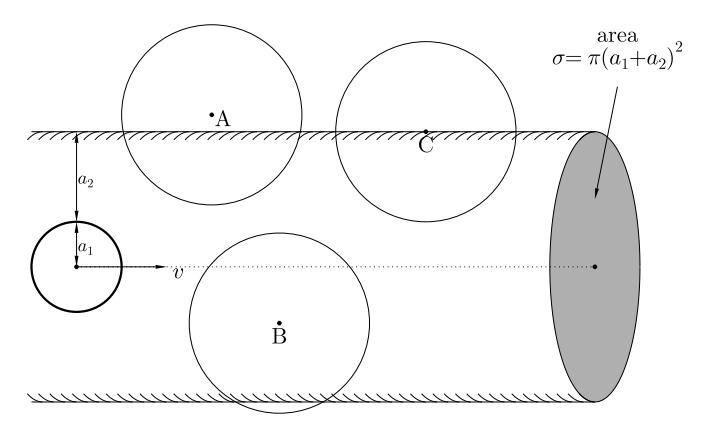
\includegraphics[width= 0.7\linewidth]{imagens/secaotransversal.png}
        \caption{Fonte: Concepts In Thermal Physics, Blundell and Blundell}
    \end{figure}

    Para o nitrogenio, \(\sigma_N = \pi(r_H + r_N)^2\) e para o oxigenio, \(\sigma_O = \pi (r_H + r_O)^2\). Como a atmosfera é feito de \(0,8 N\) e \(0,2 O\), é valido que 

    \[\sigma \equiv S_a = 0,2\sigma_O + 0,8\sigma N\]

    Assim, temos 

    \[\boxed{\lambda = \frac{1}{\sqrt{2}n(0,8\sigma_0 + 0,2\sigma_0)}}\]

    \item Assumindo que a particula perde todo seu momento ao colidir com uma molécula de ar, temos \(\delta p = mv_{rms}\). Cada colisção acontece em um tempo \(\delta t =\tau\), assim, 
    \[F = \frac{\delta p }{\delta t} = \frac{mv_{rms}}{\tau} = nS_a v_{rms}^2 \  \boxed{ = 3nS_a k_BT}\]

    \item Utilizando a definição de pressão 
    
    \[P = \frac{F}{\S_w} = \ \boxed{3n\frac{S_a}{S_w}k_B T} \]

    \item Utilizando a equação do equilíbrio hidrostático 
    
    \[\frac{dP}{dr} = -\rho g\]

    Como \(\rho\) e \(g\) são constantes, 

    \[P = -\rho g \int_h^0dh= \ \boxed{\rho g h}\]

    Onde \(h\) é a espessura da atmosfera.

    \item Igualando as pressões, 

    \[\rho g h = 3\frac{S_a}{S_w}nk_BT\]

    Resolvendo paar \(T\), temos 

    \[T = \frac{\rho g h}{3nk_B}\frac{S_w}{S_a}\]

    Como \(n\) é a densidade numérica de particulas e \(\rho\) é a densidade de massa, temos \(\rho/n = m\), assim

    \[\boxed{T= \frac{m g h}{3k_B}\frac{S_w}{S_a}}\]

    \item Fazendo uma média ponderada, 
    
    \[\boxed{m = 0,8 m_N + 0,2 m_O}\]

    \item a força que o eletron sente é dada por, 
    
    \[F = \frac{Ze^2}{4\pi \epsilon_0r^2}\]

    Igualando esta a força centrípeta

    \[\frac{Ze^2}{4\pi \epsilon_0r^2} = m_e \omega^2 r\]

    Porém, pela definição de momento angular, Temos

    \[L = m_er^2\omega \rightarrow \omega = \frac{L}{m_er^2} = \frac{n\hbar}{m_er^2}\]

    Substituindo na expressão anterior 

    \[\frac{Ze^2}{4\pi\epsilon_0 r^2} = m_e \left(\frac{n\hbar}{m_er^2}\right)^2 r\]

    Resolvendo para \(r\), 

    \[r = \frac{4\pi\epsilon_0 n^2\hbar ^2}{Z e^2 m_e}\]

    \item Para a água, temos, \(r_w = 2r_H + r_O\) e para o ar, \(r_a = 2(r_N + r_O)\), como \(S_i \propto r_i^2\), temos 
    
    \[\frac{S_w}{S_a} = \frac{(2r_H + r_O)^2}{4(r_N + r_O)^2}\]

    Assumindo que todos os elétrons estão no nível mais baixo (\(n=1\)), que \(Z_H = 1, \ Z_N = 7, \ Z_O = 8\) e que \(r\propto 1/Z\), temos 
    
    \[\boxed{\frac{S_w}{S_a}=\frac{(2/Z_H + 1/Z_O)^2}{4(1/Z_N + 1/Z_O)^2} \approx 15,73}\]

    \item Substituindo na fórmula, 

    \[T = \frac{(2\cdot 14 + 2 \cdot 16) \cdot 1,67 \cdot 10^{-27} \cdot 10^{5} \cdot 15,73}{3 \cdot 1,38\cdot 10^{-23}} \ \boxed{\approx 380\text{ K}}\]

    O que é uma estimativa bastante coerente com a relaidade, \(T = 373\) K.
\end{alternativas}
    



    
    
\end{pssolution*}
\end{pproblem}

\pts{3}
\begin{pproblem} (Adaptado Iran Problem Set)
    Dr. Shahram Abbassi é um dos cientistas iranianos mais reconhecidos no campo dos discos de acreção. Em uma de suas pesquisas recentes sobre a gigantesca nuvem molecular B32, ele descobriu uma estrela semelhante ao Sol no centro dessa nuvem específica. Segundo suas pesquisas, essa nuvem possui uma massa de $10^6 M_\odot$, um raio de $30 \, \text{pc}$ e uma viscosidade muito alta, tão grande que, se a nuvem entrasse em colapso, todo o sistema colapsaria com simetria esférica.

    O mais importante é calcular o calor específico a volume constante ($C_v$) para essa nuvem. Com base nos dados fornecidos e utilizando aproximações razoáveis, determine um limite para $C_v$ de modo que a acreção seja possível. Esses valores variam dependendo da massa e do raio da núvem? O que podemos concluir com o resultado?
\begin{pssolution*}{}{}
    Esse limite será dado pelo teorama do virial, quando, 

    \[\langle U \rangle = -2 \langle K \rangle\]

    Podemos modelar a nuvem como um gás, de modo que sua energia cinética seja dada por \(\frac{3}{2} N k_B T\). A sua energia potêncial é eneriga potencial de uma esfera, dada por \(U = -3GM^2/5R\). Assim

    \[\frac{3GM^2}{5R} = 3\frac{M}{m_p}k_B T\]

    Onde \(m\) é a massa de uma partícula da núvem.

    Desse modo, 

    \[T = \frac{GMm_p}{5k_B R}\]

    Em função do calor específico a volume consatnte, a energia é dada por, 

    \[M C_v T\]

    Voltando a igualdade, 

    \[C_v = \frac{3GM}{5R T}\]

    Substituindo \(T\), 

    \[\boxed{C_v = \frac{k_B }{m} \approx 4.1 \cdot 10^3 \text{ J kg\(^{-1}\) K\(^{-1}\)}}\]

    Note que esse valor depende apenas da massa das partículas que compões a núvem de gás. Para uma compostade hidrogênio, o valor é Surpreendentemente proximo do valor da água \(C_{v, agua} = 4,2\cdot 10^{3}\) J/kg K. 
\end{pssolution*}
\end{pproblem}


\end{document}